\section{导论}%
\label{sec:导论}
\begin{notation}
    机器学习的流程:

    1. 确立目标

    2. 收集数据

    3. 数据预处理
    
    4. 数据分析

    5. 模型训练

    6. 模型评估优化

    7. 预测
\end{notation}

机器学习和人工智能的关系:
\begin{center}
    \begin{tikzpicture}
        \draw [] (0,0) circle [radius=2] node at(0,0) {$\text{深度学习}$};
        \draw [] (0,0) circle [radius=4] node at(2,2) {$\text{机器学习}$};
        \draw [] (0,0) circle [radius=6] node at(3.5,3.5) {$\text{人工智能}$};
    \end{tikzpicture}
\end{center}

机器学习算法包含:无监督学习、监督学习、强化学习
\subsection{监督学习}%
\label{sub:监督学习}
\begin{notation}
    机器学习选择数据要求:

    1. 了解数据类型、属性、量纲

    2. 分析分布特性

    3. 选择高可信度数据

    4. 进行数据表征(将原始数据转换为计算机可识别数据)
\end{notation}
\begin{eg}
    医药领域对小分子、蛋白质、核酸进行特征数字化方法
\end{eg}
\subsubsection{数据挖掘}%
\label{subsub:数据挖掘}
1. 通过数据分析与统计学规律

2. 通过爬虫与自动化程序
\subsubsection{数据选择}%
\label{subsub:数据选择}
通过一部分数据来体现总体数据
\subsubsection{数据表征}%
\label{subsub:数据表征}
\begin{eg}
    分子指纹:

    首先提取分子结构特征(官能团等),使用分子结构特征生成比特向量,每个比特元素对应一种分子片段,通过对比比特向量的相似度来记录分子特征

    分子指纹分类:基于子结构、拓扑或路径、药效集团的分子指纹和圆形分子指纹
\end{eg}

\begin{notation}
    SMILES/简化分子线性输入规范:

    SMILES是一种ASCII字符串,具体规则如下
\end{notation}
{\centering{\subsection*{SMILES RULE}%
\label{sub:SMILES RULE}}}
\subsubsection*{1. 简单规则}%
\label{subsub:1-简单规则}
原子:原子缩写符号
\begin{eg}
    Au, Pt, C, N
\end{eg}
离子:原子加上电荷数,外接中括号
\begin{eg}
    $\text{Fe}^{3+}$: [Fe+++]

    $\text{C}^{-}$ : [C-]

    $\text{Pt}^{6+}$ : [Pt++++++]
\end{eg}
H原子:省略

相邻原子:直接连接
\begin{eg}
    Dodecane: CCCCCCCCCCCC (12 Carbons)
\end{eg}
分支:以小括号表示
\begin{eg}
    Write in git style:
    \begin{center}
        \begin{tikzpicture}
            \draw [] (-2,0)--(0,0);
            \draw [] (0,0)--(2,0);
            \draw [] (2,0)--(4,0);
            \draw [] (0,0)--(1,2);
            \draw [] (1,2)--(3,2);
            \draw [] (3,2)--(5,2);
            \filldraw [color=white] (-2,0) circle [radius=0.5] node at(-2,0) {$ $};
            \filldraw [color=white] (0,0) circle [radius=0.5] node at(0,0) {$ $};
            \filldraw [color=white] (2,0) circle [radius=0.5] node at(2,0) {$ $};
            \filldraw [color=white] (4,0) circle [radius=0.5] node at(4,0) {$ $};
            \filldraw [color=white] (1,2) circle [radius=0.5] node at(1,2) {$ $};
            \filldraw [color=white] (3,2) circle [radius=0.5] node at(3,2) {$ $};
            \filldraw [color=white] (5,2) circle [radius=0.5] node at(5,2) {$ $};
            \node at(-2,0) {$A$};
            \node at(0,0) {$B$};
            \node at(2,0) {$C$};
            \node at(4,0) {$D$};
            \node at(1,2) {$E$};
            \node at(3,2) {$F$};
            \node at(5,2) {$G$};
        \end{tikzpicture}
    \end{center}
    SMILES: AB(EFG)CD
    
\end{eg}
单键:直接省略

双键:“=”

三键:“\#”

芳香键=单键(直接省略)
\begin{notation}
    部分软件芳香键使用单双键交替表示

    芳香原子使用小写字母
\end{notation}
\begin{eg}
    hex-2-en-4-yne/戊-2-烯-4-炔(不分顺反):CC=CC\#CC

    toluene: Cc1ccccc1
\end{eg}
\subsubsection*{2. 立体结构}%
\label{subsub:2-立体结构}
环状结构:将环断开形成线性结构,以数字标记断开的原子
\begin{eg}
    Cyclohexane: C1CCCCC1
\end{eg}
同位素:[核电荷数+元素符号]
\begin{eg}
    $^{13}\text{C}$: [13C]
\end{eg}
Z/E构象:使用“/”和“$\backslash$”代表单键方向
\begin{eg}
    (2E)-hex-2-en-4-yne: C/C=C/C\#CC

    (2Z)-hex-2-en-4-yne: C/C=C$\backslash$C\#CC
\end{eg}
手性异构:@表示S,@@代表R
\begin{eg}
\begin{figure}[htpb]
    \centering
    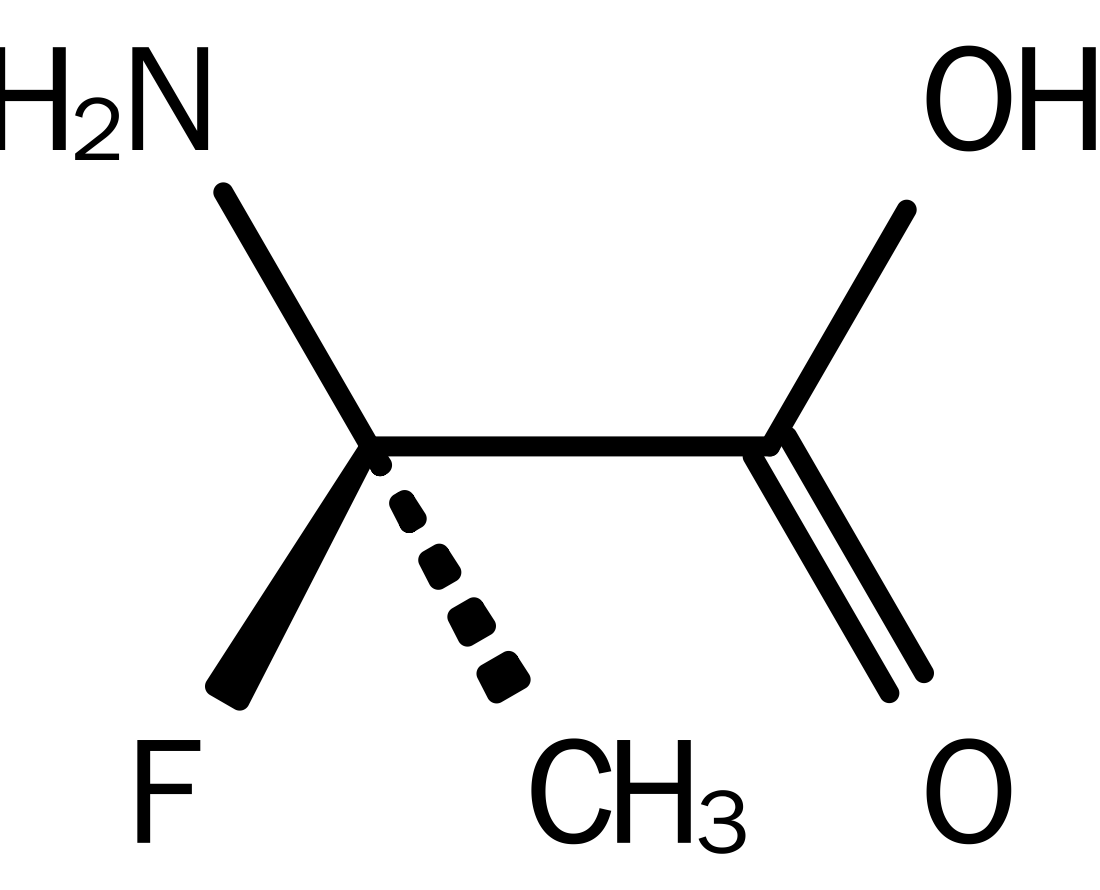
\includegraphics[width=0.2\textwidth]{fig/S&R}
    \caption{S\&R}
    \label{fig:fig-S-R}
\end{figure}
$-\text{CH}_{3}$最小,放在最后,对基团大小比较:
\[
    \text{F}>\text{NH}_{2}>\text{COOH}
.\] 
为R构型,即:N[C@@](F)(C)C(=O)O
\end{eg}
\subsubsection*{3. 算法与生成}%
\label{subsub:3-算法与生成}
\begin{notation}
    大部分SMILES生成算法为商业算法,如Morgan算法、Canonical SMILES算法等

    生成SMILES主要使用深度优先搜素(DFS)算法遍历分子图
\end{notation}



\begin{notation}
    InChI: 国际化合物标识,是规范的线性表示法、基于规范命名法则的唯一标识符

    通过分层符号“/”将表示小分子的字符串分层,前三层简化连接表的信息,其他层处理额外问题
\end{notation}
{\centering{\subsection*{InChI RULE}%
\label{sub:InChI RULE}}}
\subsubsection*{1. 主层}%
\label{subsub:1. 主层}
主层可包括三个子层:化学式、原子连接、氢原子
\[
    \text{主层}
    \begin{cases}
        \text{化学式}\\
        \text{原子连接}\\
        \text{氢原子}
    \end{cases}
.\] 


